%----------------------------%
%                            %
%      Report Template       %
%                            %
%            !!!             %
%        Compile with        %
%    XeLaTeX or LuaLaTeX     %
%            !!!             %
%                            %
%----------------------------%

\documentclass[onecolumn, letter paper]{report}
\usepackage{project}

\addbibresource{paper.bib}

\begin{document}

\maketitle

\chapter{Summary}
There are many, wildly different approaches to robotic control.
Underactuated robots are systems for which it is not possible to dictate arbitrary accelerations to all joints. Hence, a controller cannot be used to override the system dynamics and force the system on a desired trajectory as it often is done in classical control techniques.
A torque-limited pendulum is arguably the simplest underactuated robotic system and thus is a suitable system to study, test and benchmark different controllers.

This repository describes the hardware (Computer-aided design (CAD) models, Bill Of Materials (BOM), etc.) required to build a
physical pendulum system and provides the software (Unified Robot Description Format (URDF) models, simulation and controller) to control it. It provides a setup for studying established and novel control methods, and targets students and researchers interested in studying underactuation.

\chapter{Statement of Need}
This repository is designed to be used in education and research. It lowers the entry barrier
for studying underactuation in real systems which is often overlooked in conventional robotics courses.
With this software package, students who want to learn about robotics, optimal control or reinforcement learning can make hands-on
experiences with hardware and software for robot control.
The dualistic approach of describing software and hardware as well as the large spectrum of control methods are outstanding features of this package in comparison to similar software such as stable baselines \autocite{stable-baselines3}, open AI gym \autocite{Brockman2016} and Drake \autocite{drake}.
Results from real experiments are provided to ensure reproducibility and evaluate novel control methods.

\chapter{Background}
This project provides an easy accessible plant for the pendulum dynamics which is built up from scratch and uses only standard libraries. The plant can be passed to a simulator object, which is capable of integrating the equations of motion and thus simulating the pendulum's motion forward in time. The simulator can perform Euler and Runge-Kutta integration and can also visualize the motion in a matplotlib animation. Furthermore, it is possible to interface a controller to the simulator which sends control a signal in form of a torque $\tau$ to the motor.

The pendulum has a stable (downward configuration) and unstable (upward configuration) fixed points. A challenge from the control point of view is to swing the pendulum up to the unstable fixed point and stabilize the pendulum in that state respecting the torque limitation.

\chapter{Mechanical Setup}

The pendulum (\autoref{fig:pendulum}) is constructed by mounting a motor to a fixed frame, attaching a rod to the motor and a weight to the other end of the rod. The motor used in this setup is the AK80-6 actuator from T-Motor \autocite{tmotors_manual}, which is a quasi direct drive with a gear ratio of 6:1 and a peak torque of 12 Nm at the output shaft.

\begin{figure}[H]
    \centering
    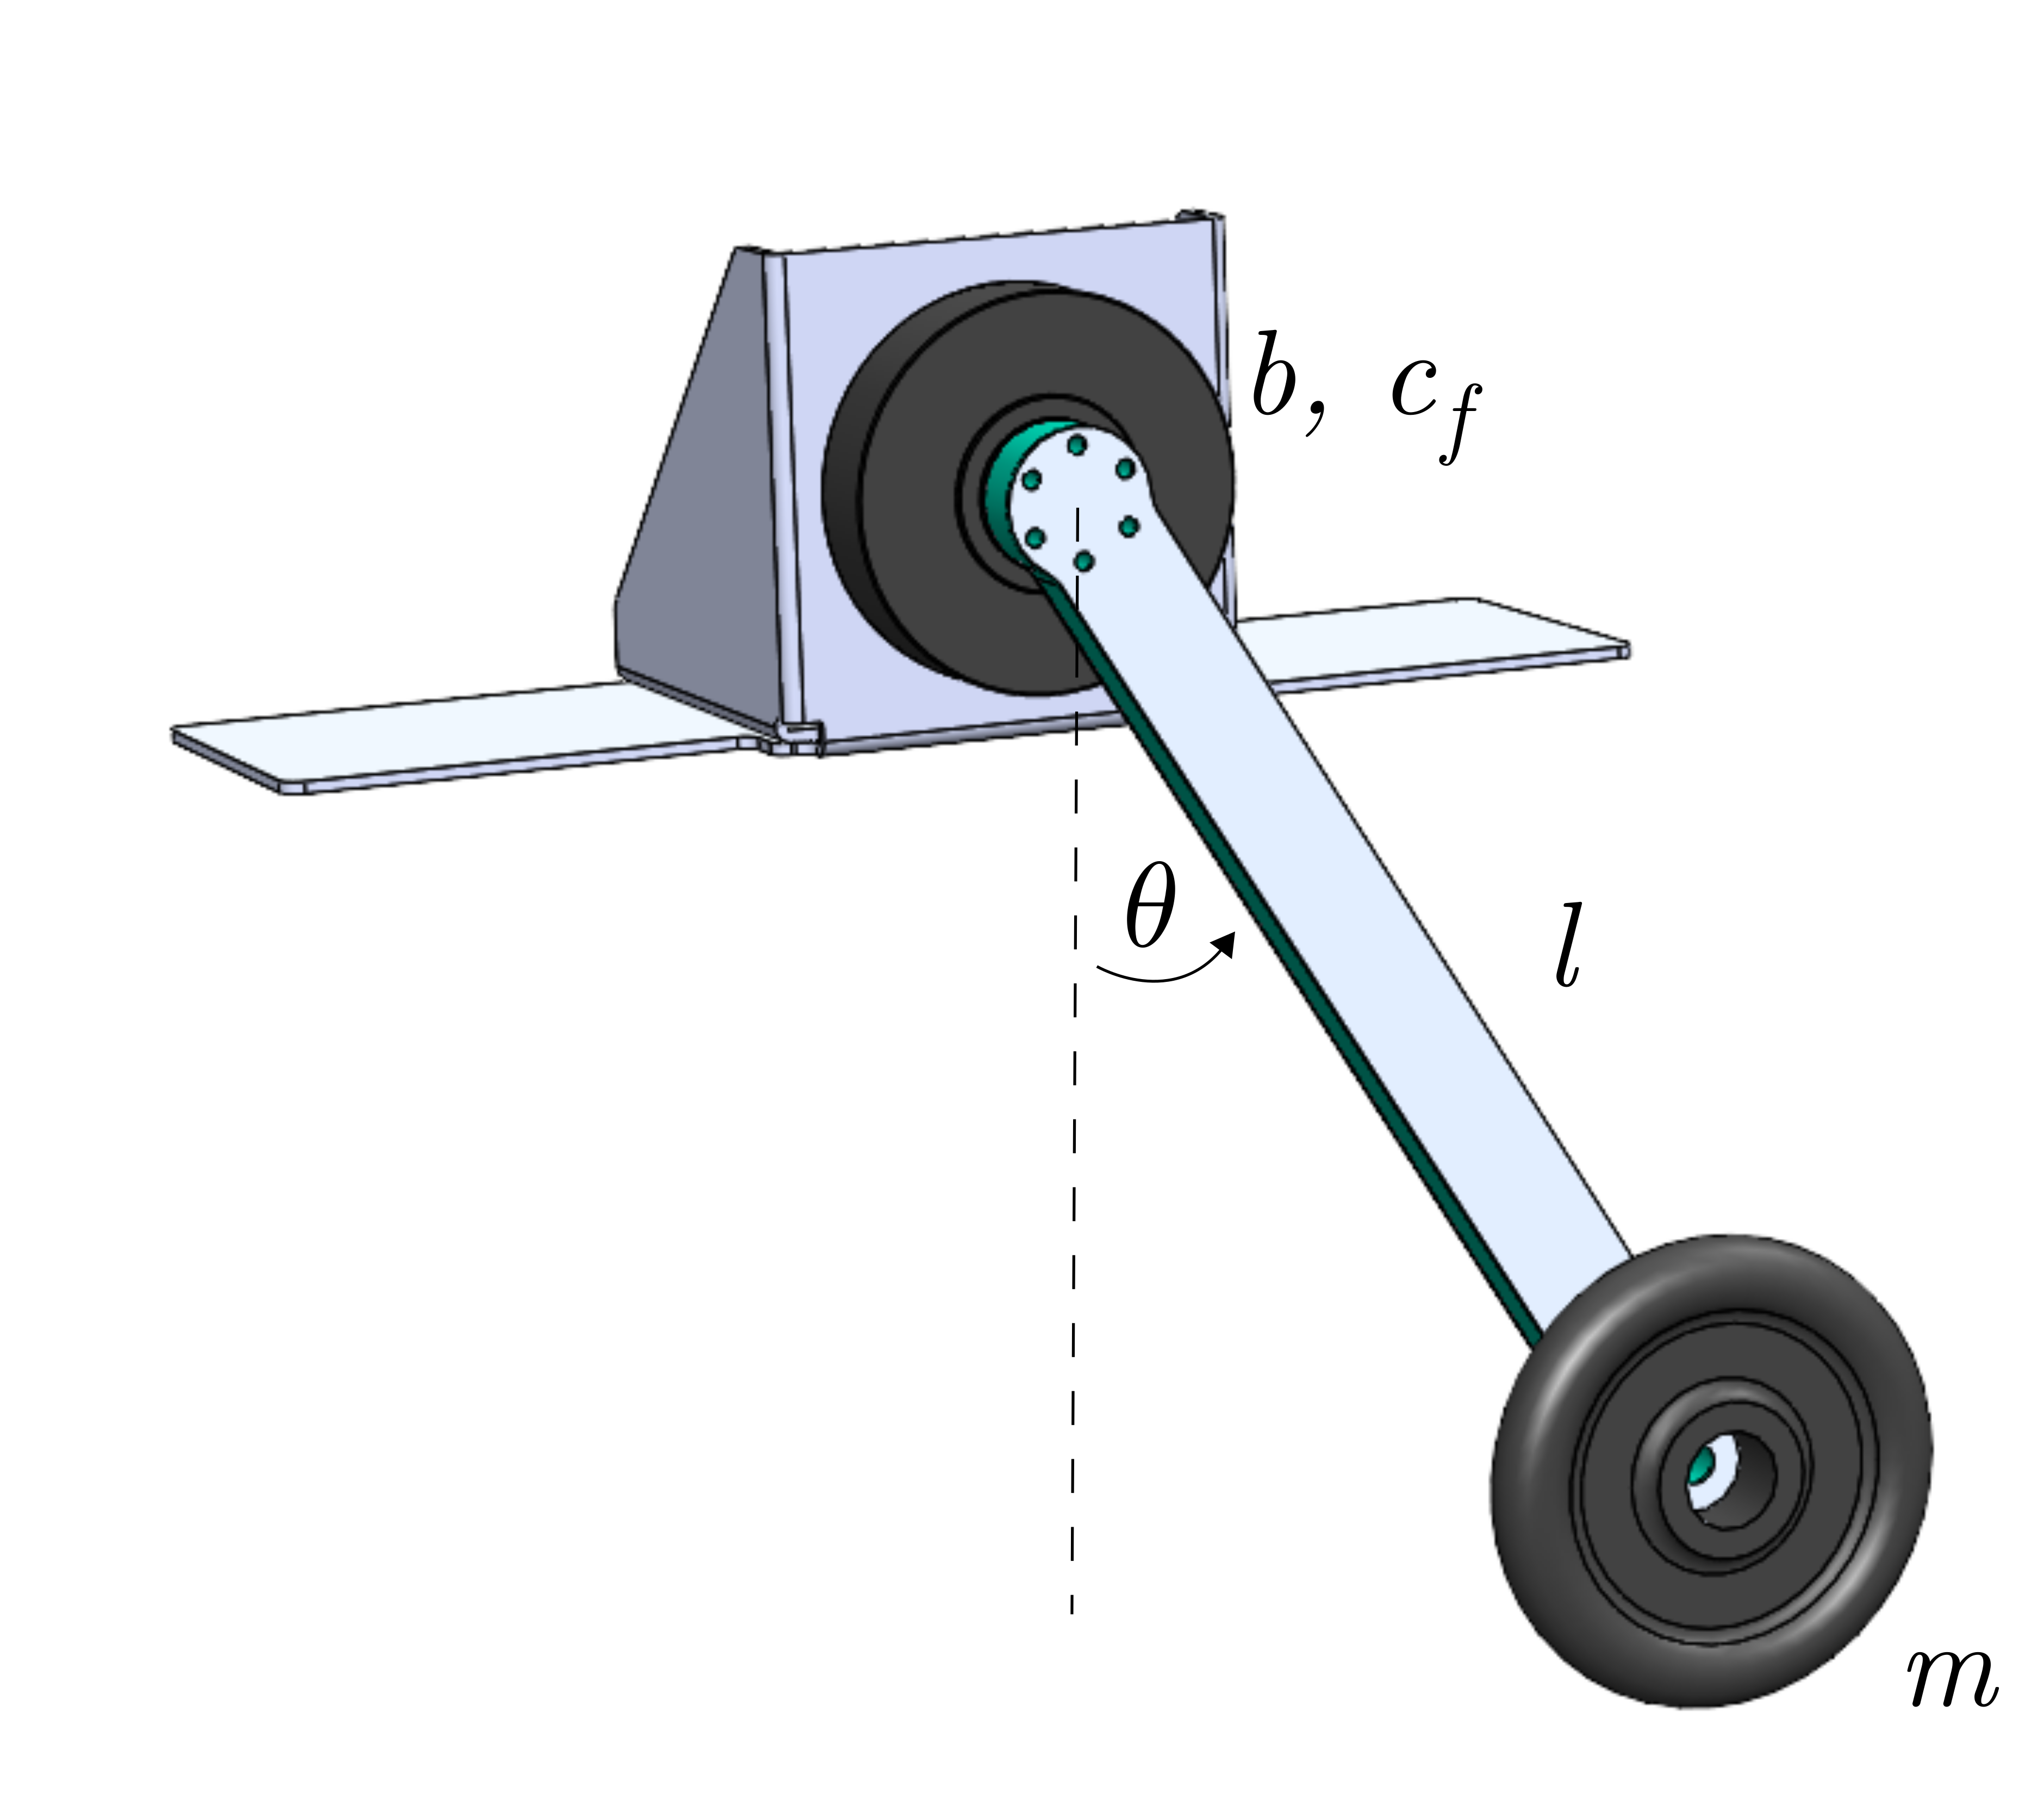
\includegraphics[width=0.4\linewidth]{figures/simple_pendulum_CAD.png}
    \caption{Simple Pendulum. The physical variables are introduced in \autoref{eq:eom}.}
    \label{fig:pendulum}
\end{figure}

\chapter{Electrical Setup}

The schematic below (\autoref{fig:electrical_schematic}) displays the electrial setup of the testbench. A main PC is connected to a motor controller board (CubeMars\_AK\_V1.1, see \cite{tmotors_manual}) mounted on the actuator. The communication takes place on a CAN bus with a maximum signal frequency of 1Mbit/sec with the 'classical' CAN protocol. Furthermore, a USB to CAN interface is needed, if the main PC doesn't feature a PCI CAN card. The actuator requires an input voltage of 24 Volts and consumes up to 24 Amps for peak torque. The power supply in our test setup is the EA-PS 9032-40 from Elektro-Automatik. The capacitor filters back EMF coming from the actuator and protects the power supply from high voltage peaks. An emergency stop button serves as additional safety measure.

\begin{figure}[H]
    \centering
    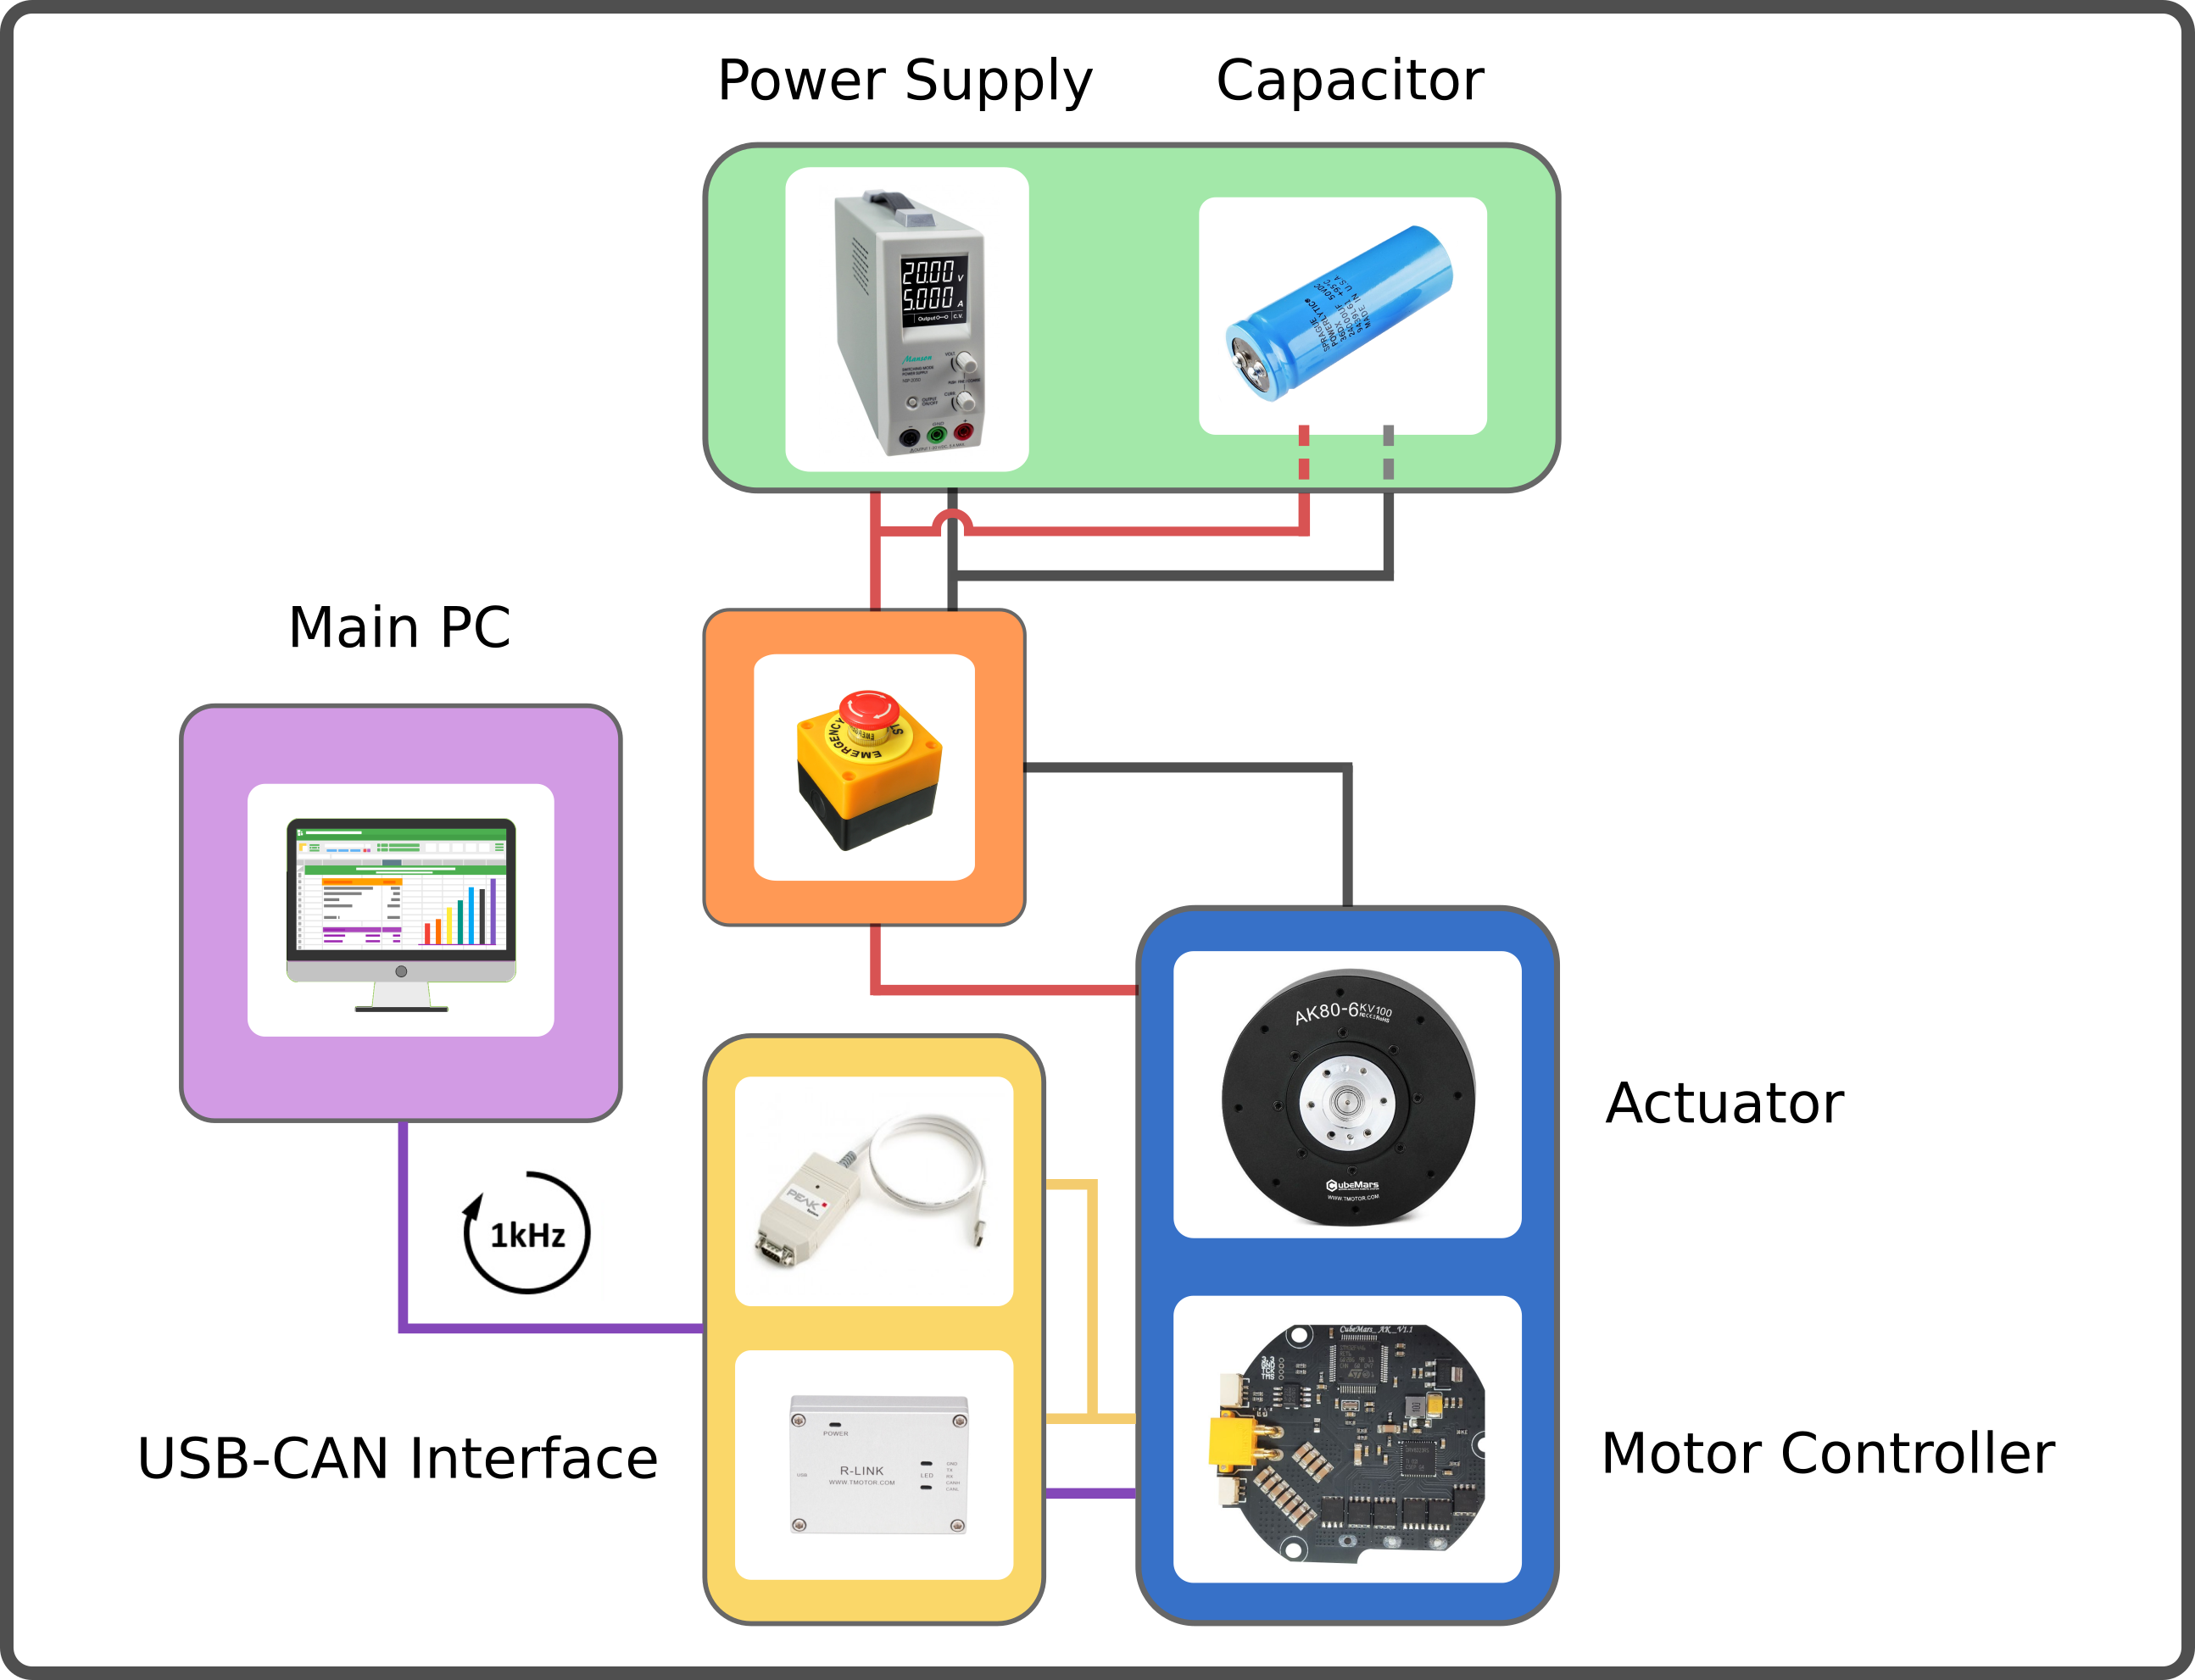
\includegraphics[width=0.4\linewidth]{figures/wiring_diagram.png}
    \caption{Electrical setup.}
    \label{fig:electrical_schematic}
\end{figure}

\chapter{Pendulum Dynamics}
The motions of a pendulum are described by the following equation of motion:

\begin{equation}
    I\ddot{\theta} + b\dot{\theta} + c_f \text{sign}(\dot{\theta}) + mgl \sin(\theta) = \tau
    \label{eq:eom}
\end{equation}

where

\begin{itemize}
    \item $\theta$, $\dot{\theta}$, $\ddot{\theta}$ are the angular displacement, angular velocity and angular acceleration of the pendulum in counter-clockwise direction. $\theta=0$ means the pendulum is at its stable fixpoint (i.e. hanging down).
    \item $I$ is the inertia of the pendulum. For a point mass: $I=ml^2$
    \item $m$ mass of the pendulum
    \item $l$ length of the pendulum
    \item $b$ damping friction coefficient
    \item $c_f$ coulomb friction coefficient
    \item $g$ gravity (positive direction points down)
    \item $\tau$ torque applied by the motor
\end{itemize}

We provide a pendulum plant model which can be used for computing trajectories and policies without the actual hardware, simulating the execution of a controller as well as simulating the systems response during real time control. Also, a system identification method is implemented which can reliably estimate the unknown pendulum parameters of the real setup.

\chapter{Control Methods}
The swing-up with a limited motor torque $\tau$ serves as a benchmark for various control algorithms. If the torque limit is set low enough, the pendulum is no longer able to simply go up to the unstable fixpoint but instead the pendulum has to swing and built up energy in the system.

\begin{figure}[H]
    \centering
    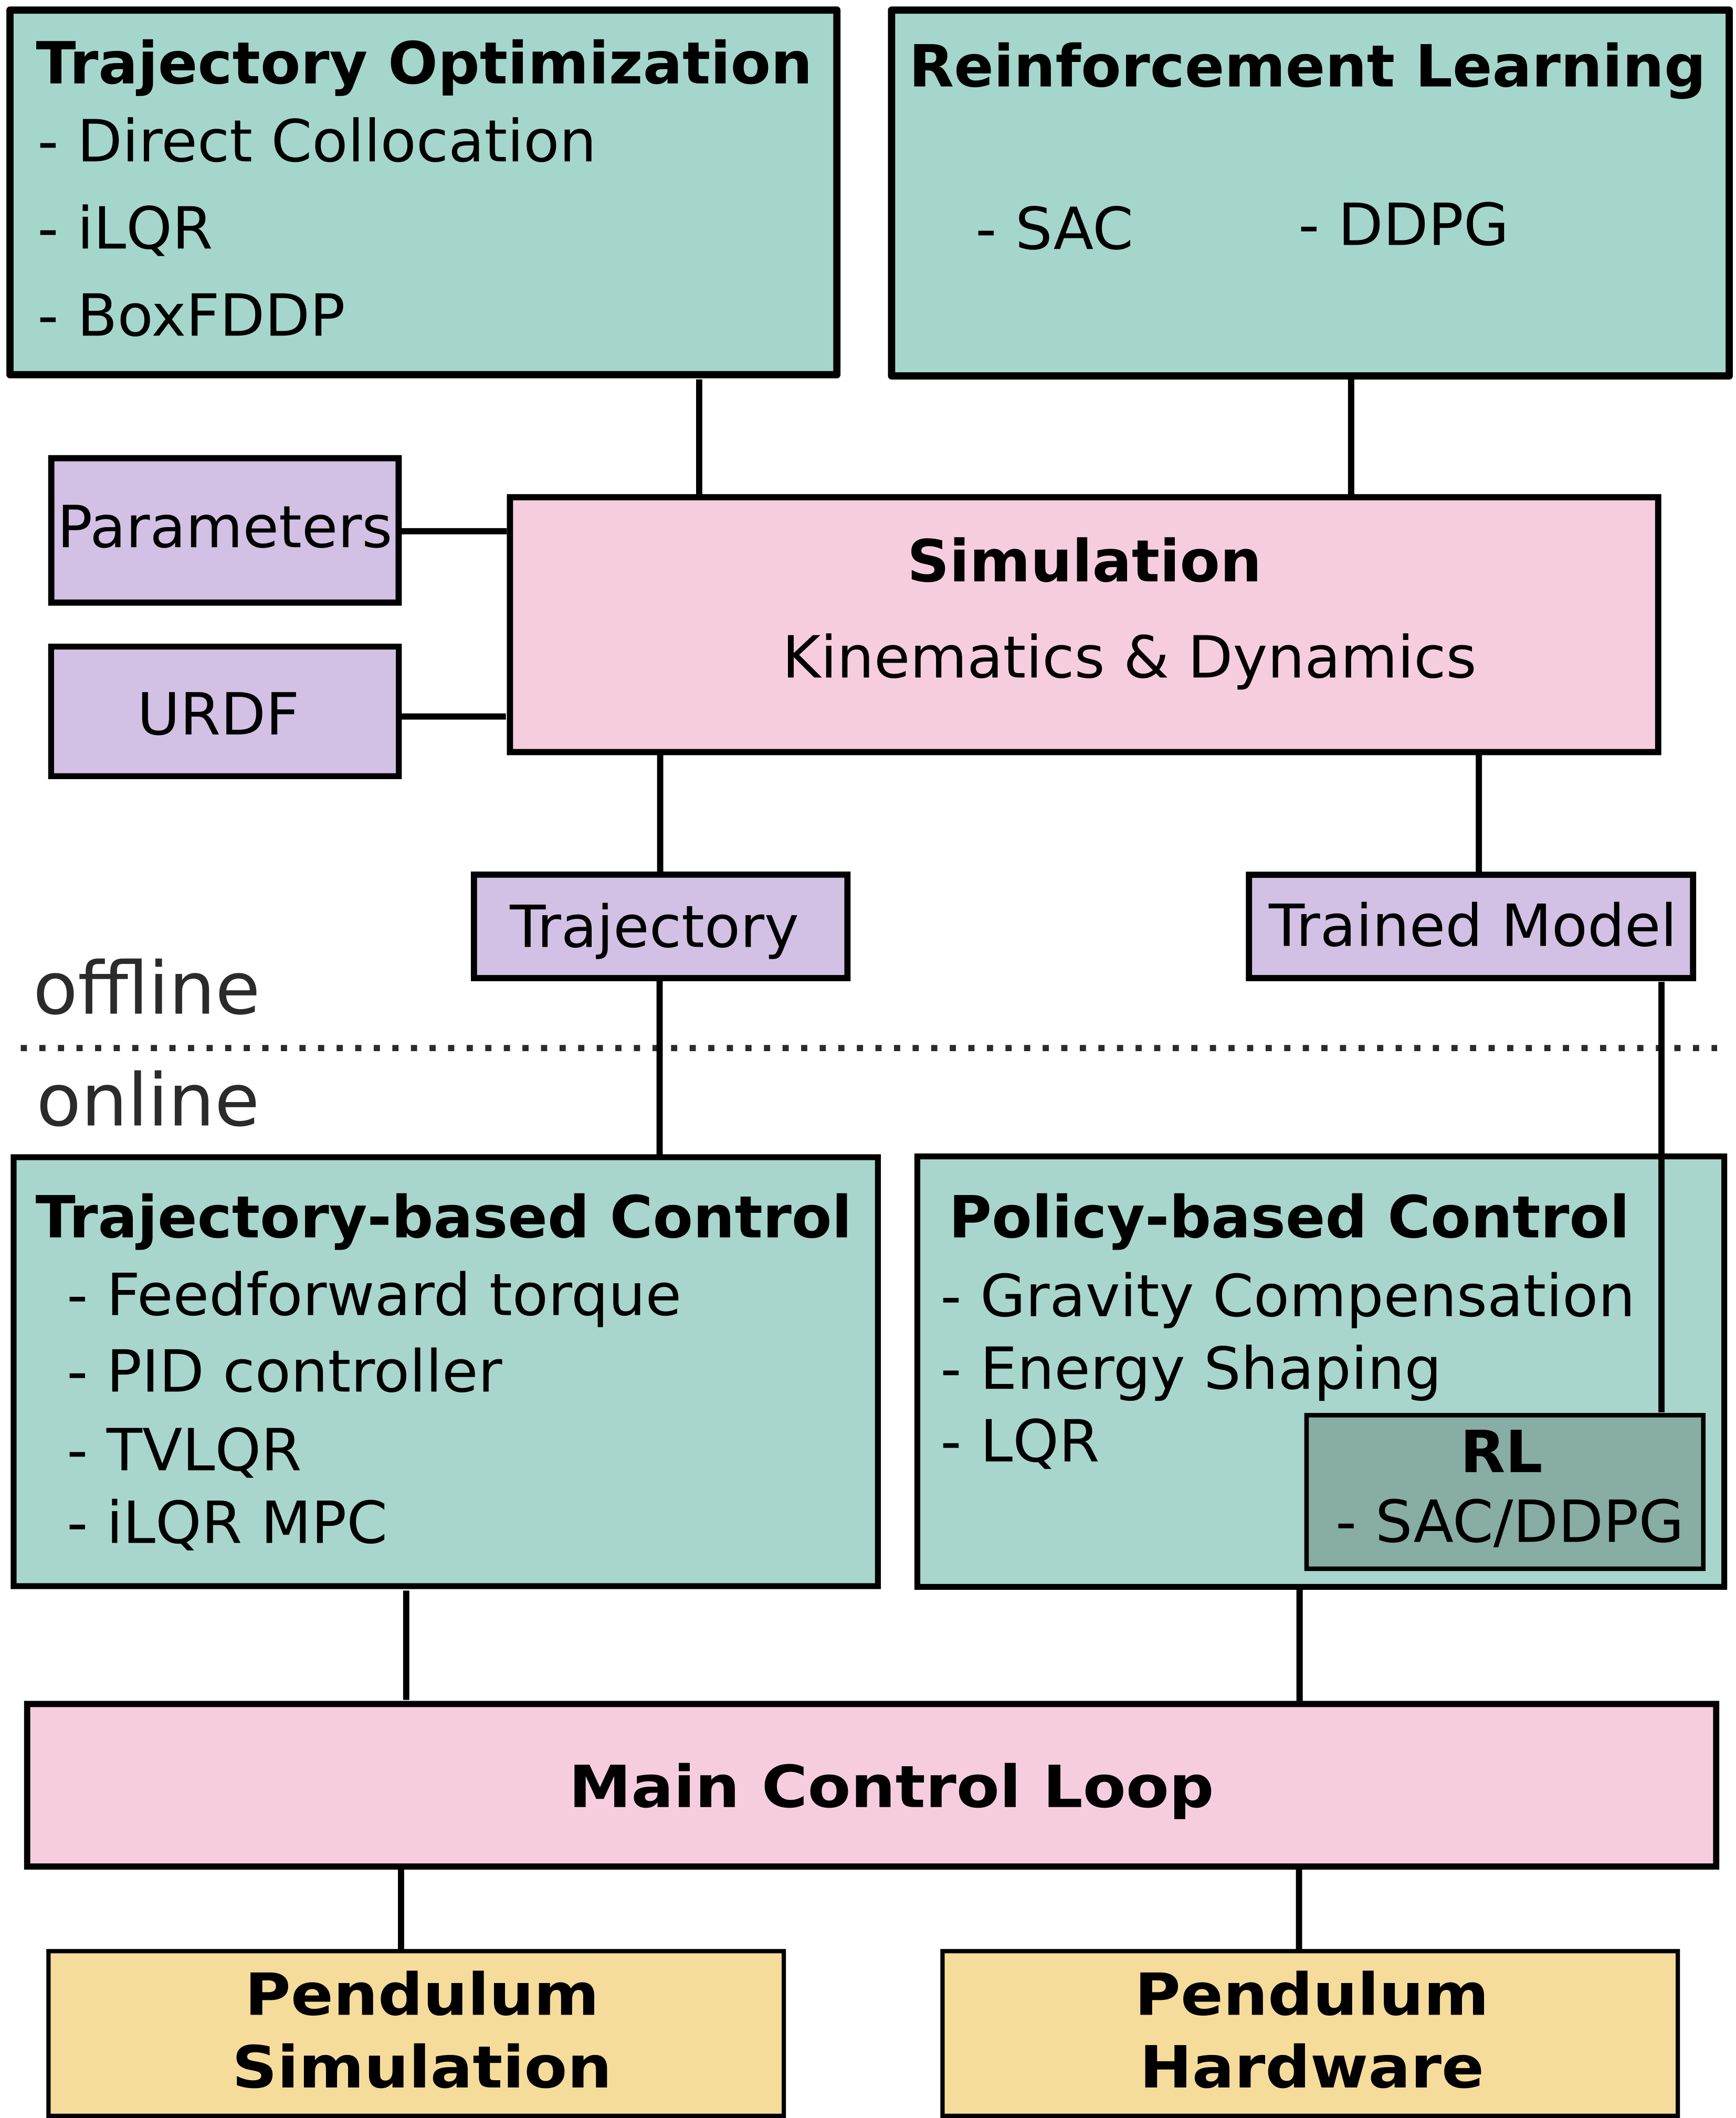
\includegraphics[width=0.4\linewidth]{figures/controller_overview.png}
    \caption{Control Software Structure.}
    \label{fig:software_structure}
\end{figure}

The control methods that are currently implemented in this library (see also \autoref{fig:software_structure}) can be grouped in four categories:

\textbf{Trajectory optimization} tries to find a trajectory of control inputs and states that is feasible for the system while minimizing a cost function. The cost function can for example include terms which drive the system to a desired goal state and penalize the usage of high torques. The following trajectory optimization algorithms are implemented:

\begin{itemize}
    \item Direct Collocation \autocite{hargraves1987direct}
    \item Iterative Linear Quadratic Regulator (iLQR) \autocite{weiwei2004iterative}
    \item Feasibility driven Differential Dynamic Programming (FDDP) \autocite{mastalli2020crocoddyl}
\end{itemize}

The optimization is done with a simulation of the pendulum dynamics.

\textbf{Reinforcement learning} (RL) can be used to learn a policy on the state space of the robot, which then can be used to control the robot. The simple pendulum can be formulated as a RL problem with two continuous inputs and one continuous output. Similar to the cost function in trajectory optimization, the policy is trained with a reward function. The following RL algorithms are implemented:

\begin{itemize}
    \item Soft Actor Critic (SAC) \autocite{haarnoja2018soft}
    \item Deep Deterministic Policy Gradient (DDPG) \autocite{lillicrap2019continuous}
\end{itemize}

Both methods, are model-free, i.e. they use the dynamics of the system as a black box. Currently, learning is possible in the simulation environment.

\textbf{Trajectory-based controllers} act on a precomputed trajectory and ensure that the system follows the trajectory properly. The trajectory-based controllers implemented in this project are:

\begin{itemize}
    \item Feedforward torque
    \item Proportional-integral-derivative (PID) control
    \item Time-varying Linear Quadratic Regulator (TVLQR)
    \item Model Predictive Control (MPC) with iLQR
\end{itemize}

Feedforward and PID controller operate model independent, while the TVLQR and iLQR MPC controllers utilize knowledge about the pendulum model. In contrast to the others, the iLQR MPC controller optimizes over a predefined horizon at every timestep.

\textbf{Policy-based controllers} take the state of the system as input and ouput a control signal. In contrast to trajectory optimization, these controllers do not compute just a single trajectory. Instead, they react to the current state of the pendulum and because of this they can cope with perturbations during the execution. The following policy-based controllers are implemented:

\begin{itemize}
    \item Energy Shaping
    \item Linear Quadratic Regulator (LQR)
    \item Gravity Compensation
\end{itemize}

All of these controllers utilize model knowledge. Additionally, the control policies, obtained by one of the RL methods, fall in the category of policy-based control.

The implementations of direct collocation and TVLQR make use of Drake \autocite{drake}, iLQR makes use of either the symbolic library of Drake or sympy, FDDP makes use of Crocoddyl \autocite{mastalli2020crocoddyl}, SAC uses stable-baselines3 \autocite{stable-baselines3} and DDPG is implemented in tensorflow \autocite{tensorflow2015-whitepaper}. The other methods use only standard libraries.
This repository is designed to welcome contributions in form of novel optimization methods/controllers/learning algorithms to extend this list.

To get an understanding of the functionality of the implemented controllers they can be visualized in the pendulum's state space. Example visualizations of the energy shaping controller and the policy learned with DDPG are shown in figure \autoref{fig:controller_plots}.

\begin{figure}[H]
    \centering
    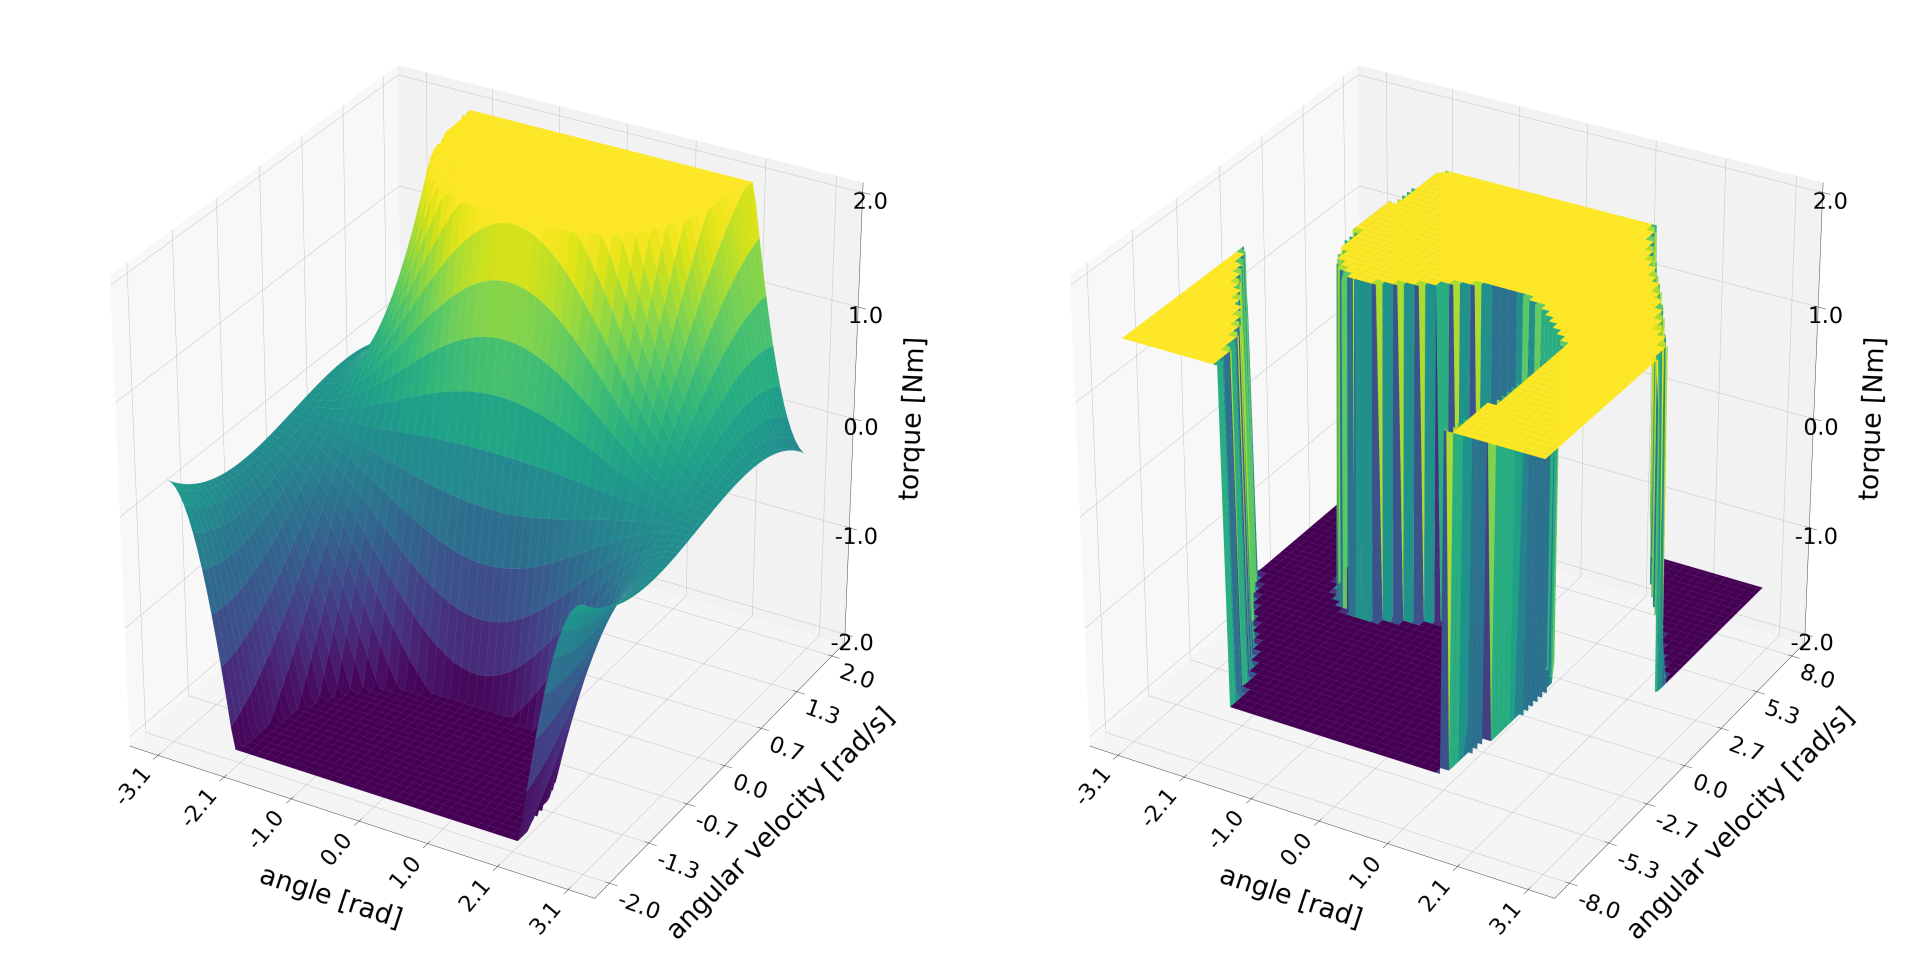
\includegraphics[width=0.6\linewidth]{figures/energy_and_ddpg.png}
    \caption{Energy Shaping Controller and DDPG Policy.}
    \label{fig:controller_plots}
\end{figure}

Furthermore, the swing-up controllers can be benchmarked in simulation, where it is evaluated how fast, efficient, consistent, stable and sensitive the controller is during the swing-up. See figure \autoref{fig:benchmark} for a comparison of the different controllers' benchmark results.

The benchmark criteria are:

\begin{itemize}
    \item \textbf{Frequency}: The inverse of the time the controller needs to process state input and return a control signal (hardware dependent).
    \item \textbf{Swingup time}: The time it takes for the controller to swing-up the pendulum from the lower fixpoint to the upper fixpoint.
    \item \textbf{Energy consumption}: The energy the controller uses during the swingup motion and holding the pendulum in position afterwards.
    \item \textbf{Smoothness}: Measures how much the controller changes the control output during execution.
    \item \textbf{Consistency}: Measures if the controller is able to drive the pendulum to the unstable fixpoint for varying starting positions and velocities.
    \item \textbf{Robustness}: Tests the controller abilities to recover from perturbations during the swingup motions.
    \item \textbf{Insensitivity}: The pendulum parameters (mass, length, friction, inertia) are modified without using this knowledge in the controller.
    \item \textbf{Reduced torque limit}: The minimal torque limit with which the controller is still able to swing-up the pendulum.
\end{itemize}

The results shown in \autoref{fig:benchmark} are the average of 100 repetitions for every controller and criterium. In the case of consistency, robustness and insensitivity the percentage refers to the ratio of successfull swingup motions of the 100 repetitions.

\begin{figure}[H]
    \centering
    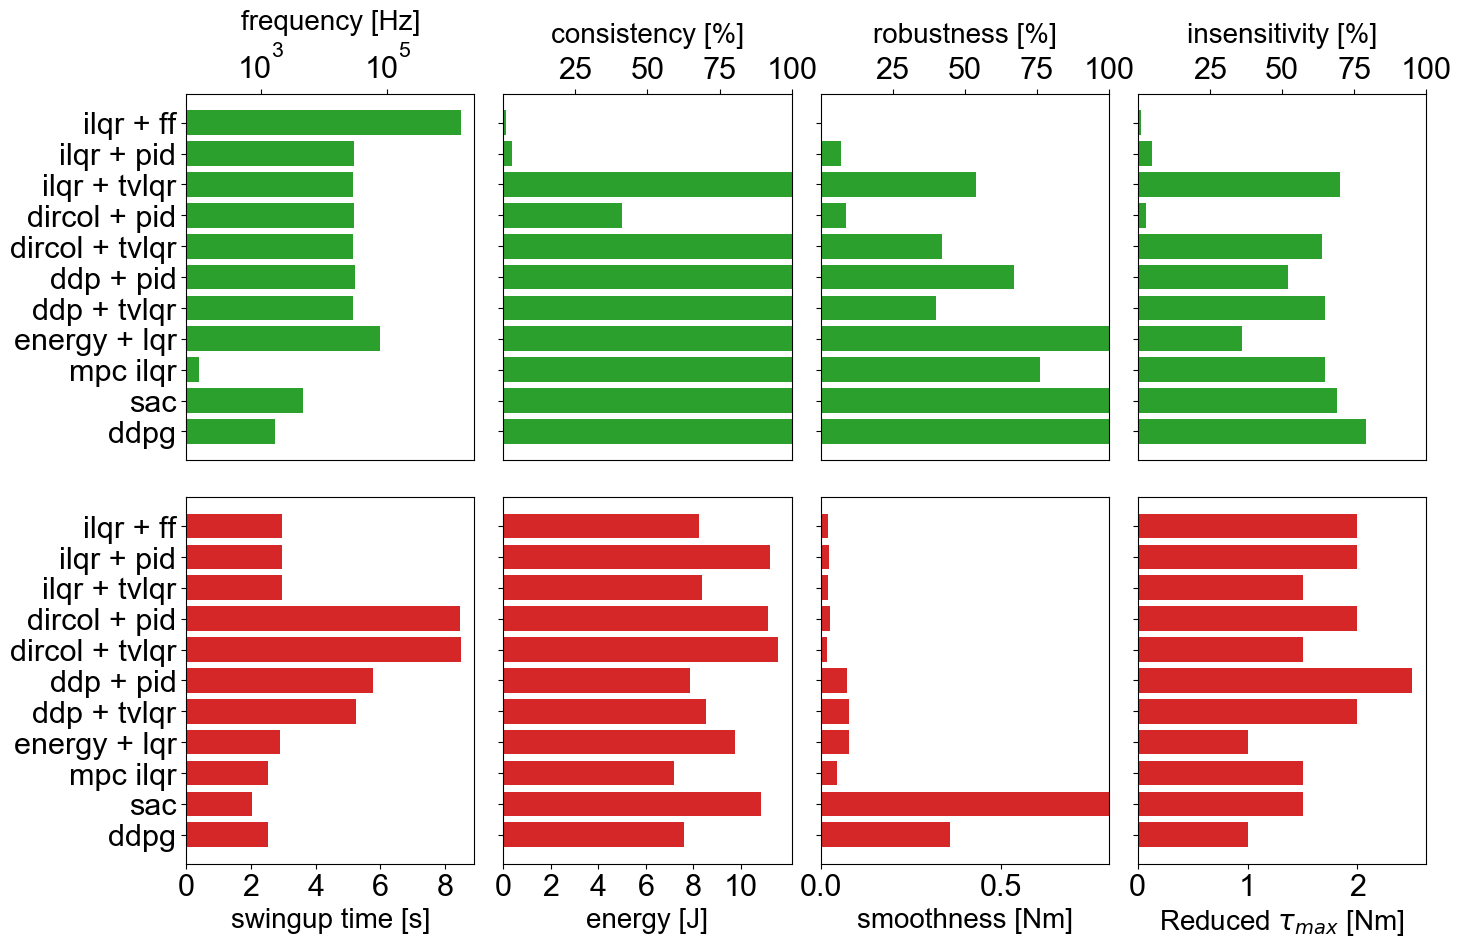
\includegraphics[width=0.8\linewidth]{figures/benchmark_barplot.png}
    \caption{Benchmark results.}
    \label{fig:benchmark}
\end{figure}

Trajectory optimization (iLQR, direct collocation, ddp) produces smooth trajectories, which swing up the pendulum relatively quickly. But they do require a trajectory following control loop (PID, TVLQR) to make them more consistent, robust and insensitive. This can become a problem for large deviations from the nominal trajectory. RL policies perform well on consistency, robustness, insensitivity and are able to perform fast swingup motions. Their drawback is that their output can fluctuate which can result in rougher motions. The model predictive iLQR controller has an overall good performance but has the disadvantage that is it comparatively slow due to the optimization at every timestep. The energy shaping plus LQR controller, despite its simplicity, shows very satisfying results in all benchmark categories.

\chapter*{Acknowledgements}

This work has been performed in the VeryHuman project funded by the German Aerospace Center (DLR) with federal funds (Grant Number: FKZ 01IW20004) from the Federal Ministry of Education and Research (BMBF) and is additionally supported with project funds from the federal state of Bremen for setting up the Underactuated Robotics Lab (Grant Number: 201-001-10-3/2021-3-2).

\printbibliography[heading=bibintoc, title={Bibliography}]

\end{document}
